\section{Algorithmenportfolios}

Der Ansatz der Algorithmenportfolios stammt ursprünglich aus der Ökonomie im Zusammenhang mit der Streuung von Investitionen. Denn obwohl die Investition in eine einzige viel versprechende Anlage hohe Gewinne erwarten lässt, birgt sie auch das Risiko eines hohen Verlustes, sollte sich die Anlage als Fehlschlag herausstellen. Um das Risiko eines solches Kapitalverlustes zu senken werden Portfolios eingesetzt. Für ein Gesamtvolumen $\mathcal{F}$ an Finanzmittel und einer Menge von Anlagen $ (a_1, a_2, ... ,  a_n) $ werden die Investitionen $ (x_1, x_2, .... , x_n),~ \sum_{i=1}^n{x_i} = \mathcal{F}, x_i \in \mathbb{Q}$ mithilfe eines Verteilungsvektors $ \vec v $ mit $ \sum_{i=1}^n{v_i} = 1, v_i \in \mathbb{Q}$ gestreut. Hauptproblem dabei ist es einen Kompromiss zwischen erwartetem Gewinn und Risiko, d. h. der Varianz des erwarteten Gewinns, zu finden \cite{markowitz1}.

Die Auswahl eines Portfolios kann in zwei Phasen unterteilt werden. Zum einen in eine Beobachtungsphase, in der der Markt betrachtet wird. Zum anderen in eine Analysephase, in der Prognosen über die Zukunft anhand der gemachten Beobachtungen berechnet werden. Die erstellten Prognosen dienen dann als Grundlage um die Portfolios zu finden, die einen optimalen Kompromiss zwischen Gewinn und Risiko bieten. Der optimale Kompromiss ist jener, der für einen bestimmten Erwartungswert die niedrigste Varianz bzw. für eine bestimmte Varianz den höchsten Erwartungswert liefert. Durch diese Betrachtung ergeben sich mehrere optimale Portfolios. Sie liegen auf der von Markovitz 'efficient frontier' benannten Linie (siehe Abbildung \ref{efficientfrontier}). Neben diesen beiden Kriterien müssen aber auch weitere Punkte beachtet werden. Beispielsweise ist auf eine Vielfalt der gewählten Anlagenbereiche zu achten, da ein einseitiges Portfolio gegen einen Einbruch der gewählten Branche anfällig wäre. \\

\begin{figure}[h]
\centering
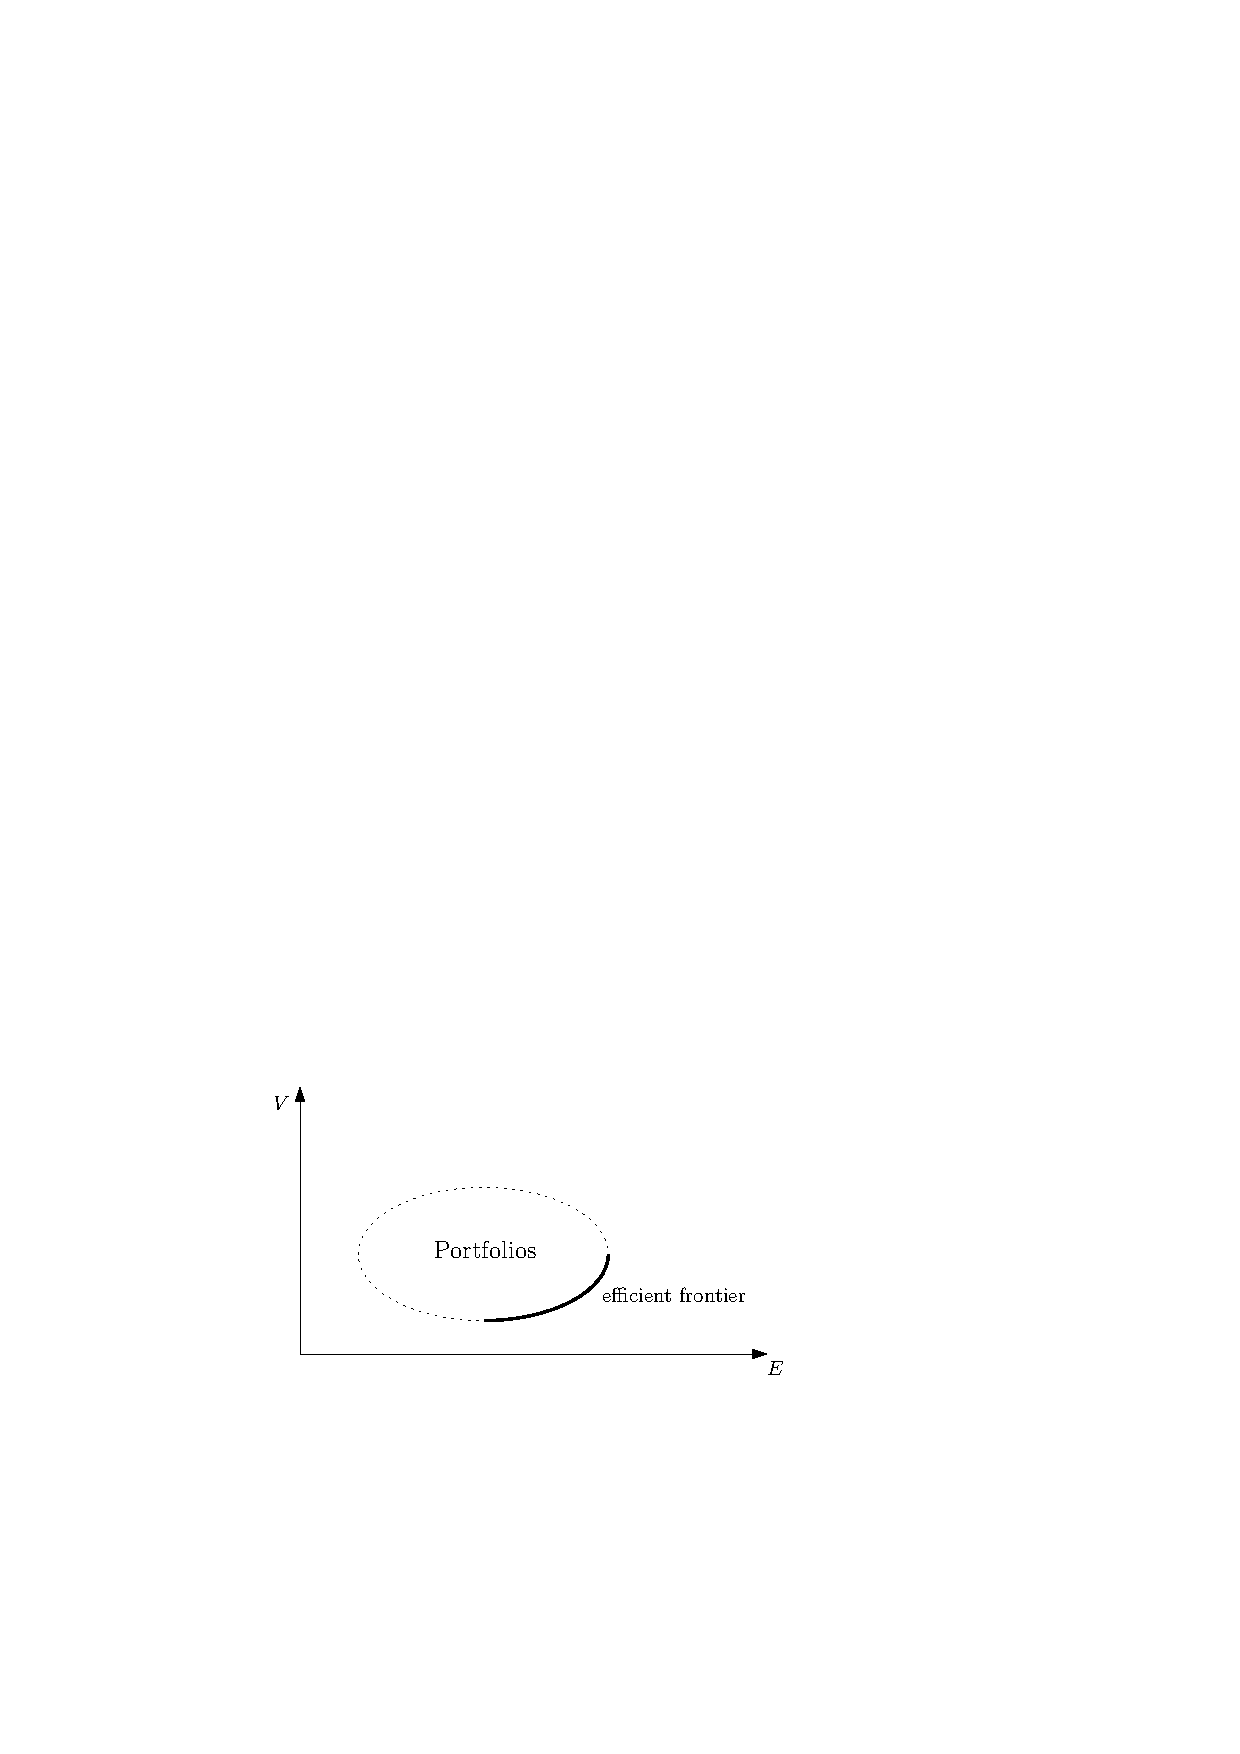
\includegraphics{efficientfrontier.pdf}
\caption[Efficient Frontier]{Innerhalb der Ellipse liegen alle möglichen Portfolios. Der markierte Rand der Ellipse ist die 'efficient frontier' auf der alle optimalen Portfolios liegen.}
\label{efficientfrontier}
\end{figure}
